\graphicspath{{content/chapters/6_implementation/figures/}}
\chapter{Implementation}
\label{chp:implementation}

\section{Datasets}
\label{sec:datasets}

Following Section~\ref{sec:variable_length_handling}, this section describes the dataset handling mechanisms implemented to accommodate variable-length audio signals. The custom dataset classes developed for this project inherit from PyTorch’s \texttt{Dataset} class and are used in both training and denoising pipelines. These implementations are central to managing waveform padding, STFT conversion, and batch preparation for deep learning models.

Each class implements three essential methods that are all similarly structured but differ in their approach to handling variable-length data. The \texttt{\_\_init\_\_} method initializes key parameters, constructs paths for clean and noisy speech files, and prepares required caches. Here the amount of parameter varies based on the approach as some methods require more configuration than others. The \texttt{\_\_len\_\_} method is a simple return function that provides the total number of samples in the dataset. The \texttt{\_\_getitem\_\_} method applies necessary transformations to the audio files such as mono conversion, resampling, and STFT. It also handles the padding and truncation of audio samples to ensure consistent input dimensions across batches. Real and imaginary STFT components are used as input-output pairs, ensuring a consistent format across all datasets. A critical motivation for this implementation is real-time deployment. The STFT inherently segments audio into short overlapping frames, simulating real-time input. This makes training models on STFT frames suitable for later real-time inference.

\subsection{Static Bucketing}
\label{subsec:static_dataset}

The first dataset implementation explored to address the variable-length issue and limitations of fixed-length padding is the static bucketing method. This approach uses a predefined set of bucket sizes, each corresponding to a fixed number of audio samples. In this project, sizes were derived by multiplying the sampling rate (48~kHz) by target durations (e.g., 1s, 2s, 3s), resulting in discrete, fixed-length buckets.

Each audio file is assigned to the first bucket that can fully contain it. For example, an audio clip of 2.5 seconds is assigned to the 3s bucket, since the 2s bucket is insufficient, and the 3s bucket is the next available option.

\begin{figure}[H]
    \centering
    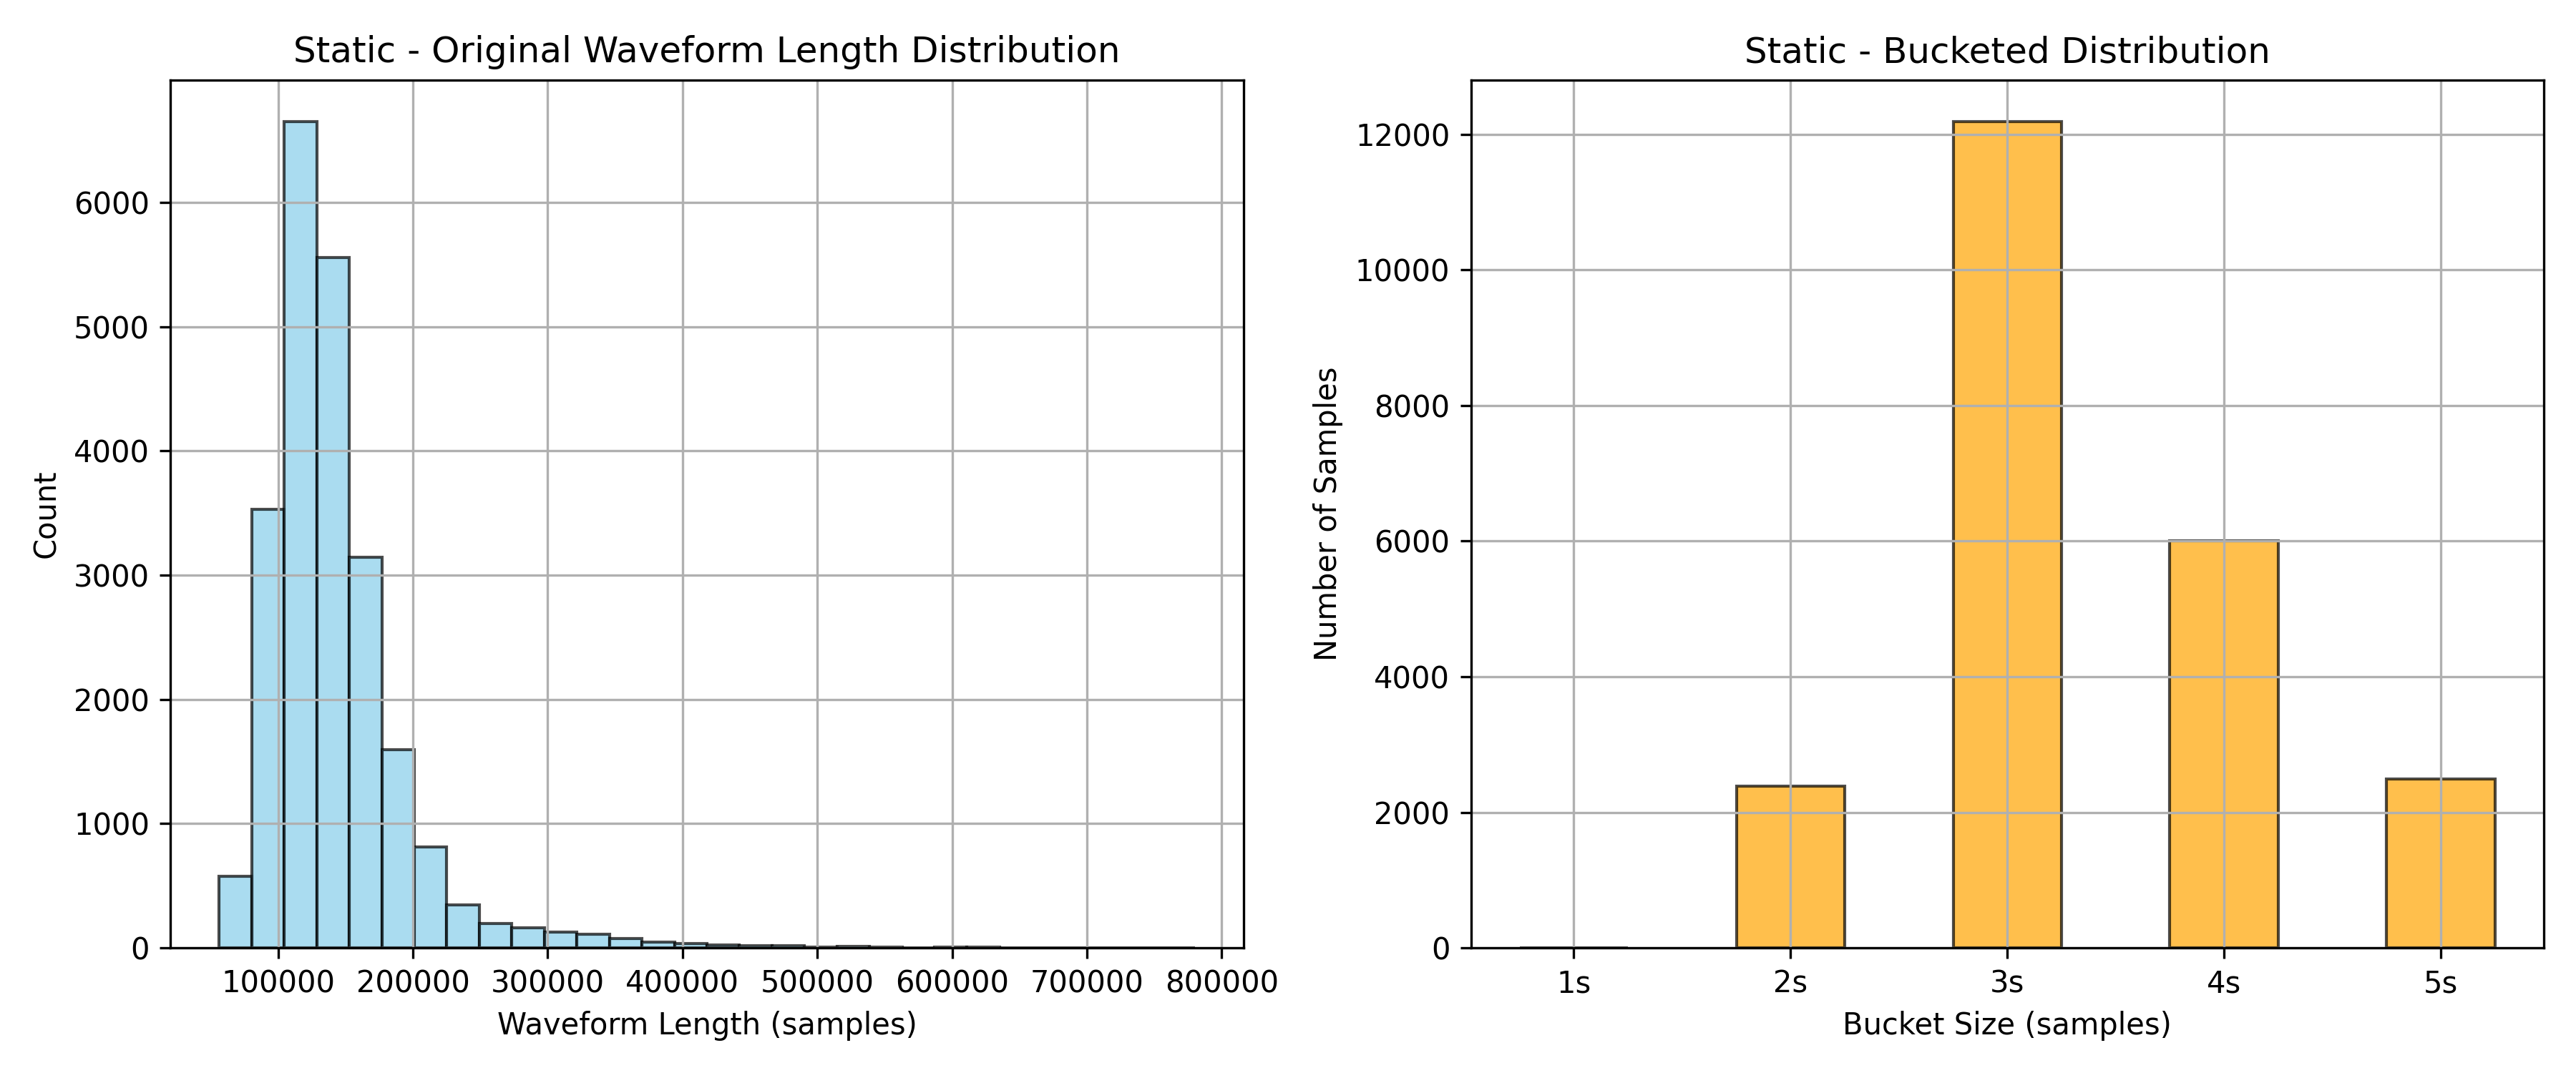
\includegraphics[width=0.9\textwidth]{static_pad.png}
    \caption{Static bucketing histogram and bucket allocation}
    \label{fig:static_pad}
\end{figure}

The \texttt{bucket\_handler} method iterates over all clean files, assigns them to buckets, and caches these assignments to avoid redundant processing in future runs. During training, a custom \texttt{collate} function pads or truncates audio waveforms to match their bucket’s target length. This guarantees consistent input dimensions within each batch, which is essential for batch-based processing in neural networks.

While static bucketing does not eliminate padding altogether, it significantly reduces the amount of excess padding compared to a naive fixed-length strategy. As shown in Figure~\ref{fig:static_pad}, most samples naturally group into the smaller buckets (3s), improving efficiency and reducing unnecessary computation.

\subsection{Dynamic Bucketing}
\label{subsec:dynamic_dataset}

The dynamic bucketing method improves upon static bucketing by adapting the bucket sizes to the actual distribution of audio file lengths. Instead of predefined durations, the method uses K-Means clustering on the waveform lengths to compute optimal bucket centers. This enables buckets that reflect the natural variance in the dataset.

During initialization, the method measures the length of each clean file and applies K-Means with a specified number of clusters (\texttt{num\_buckets}). These cluster centers become the bucket sizes, and each sample is assigned to the closest one. Like static bucketing, this assignment is cached.

\begin{figure}[H]
    \centering
    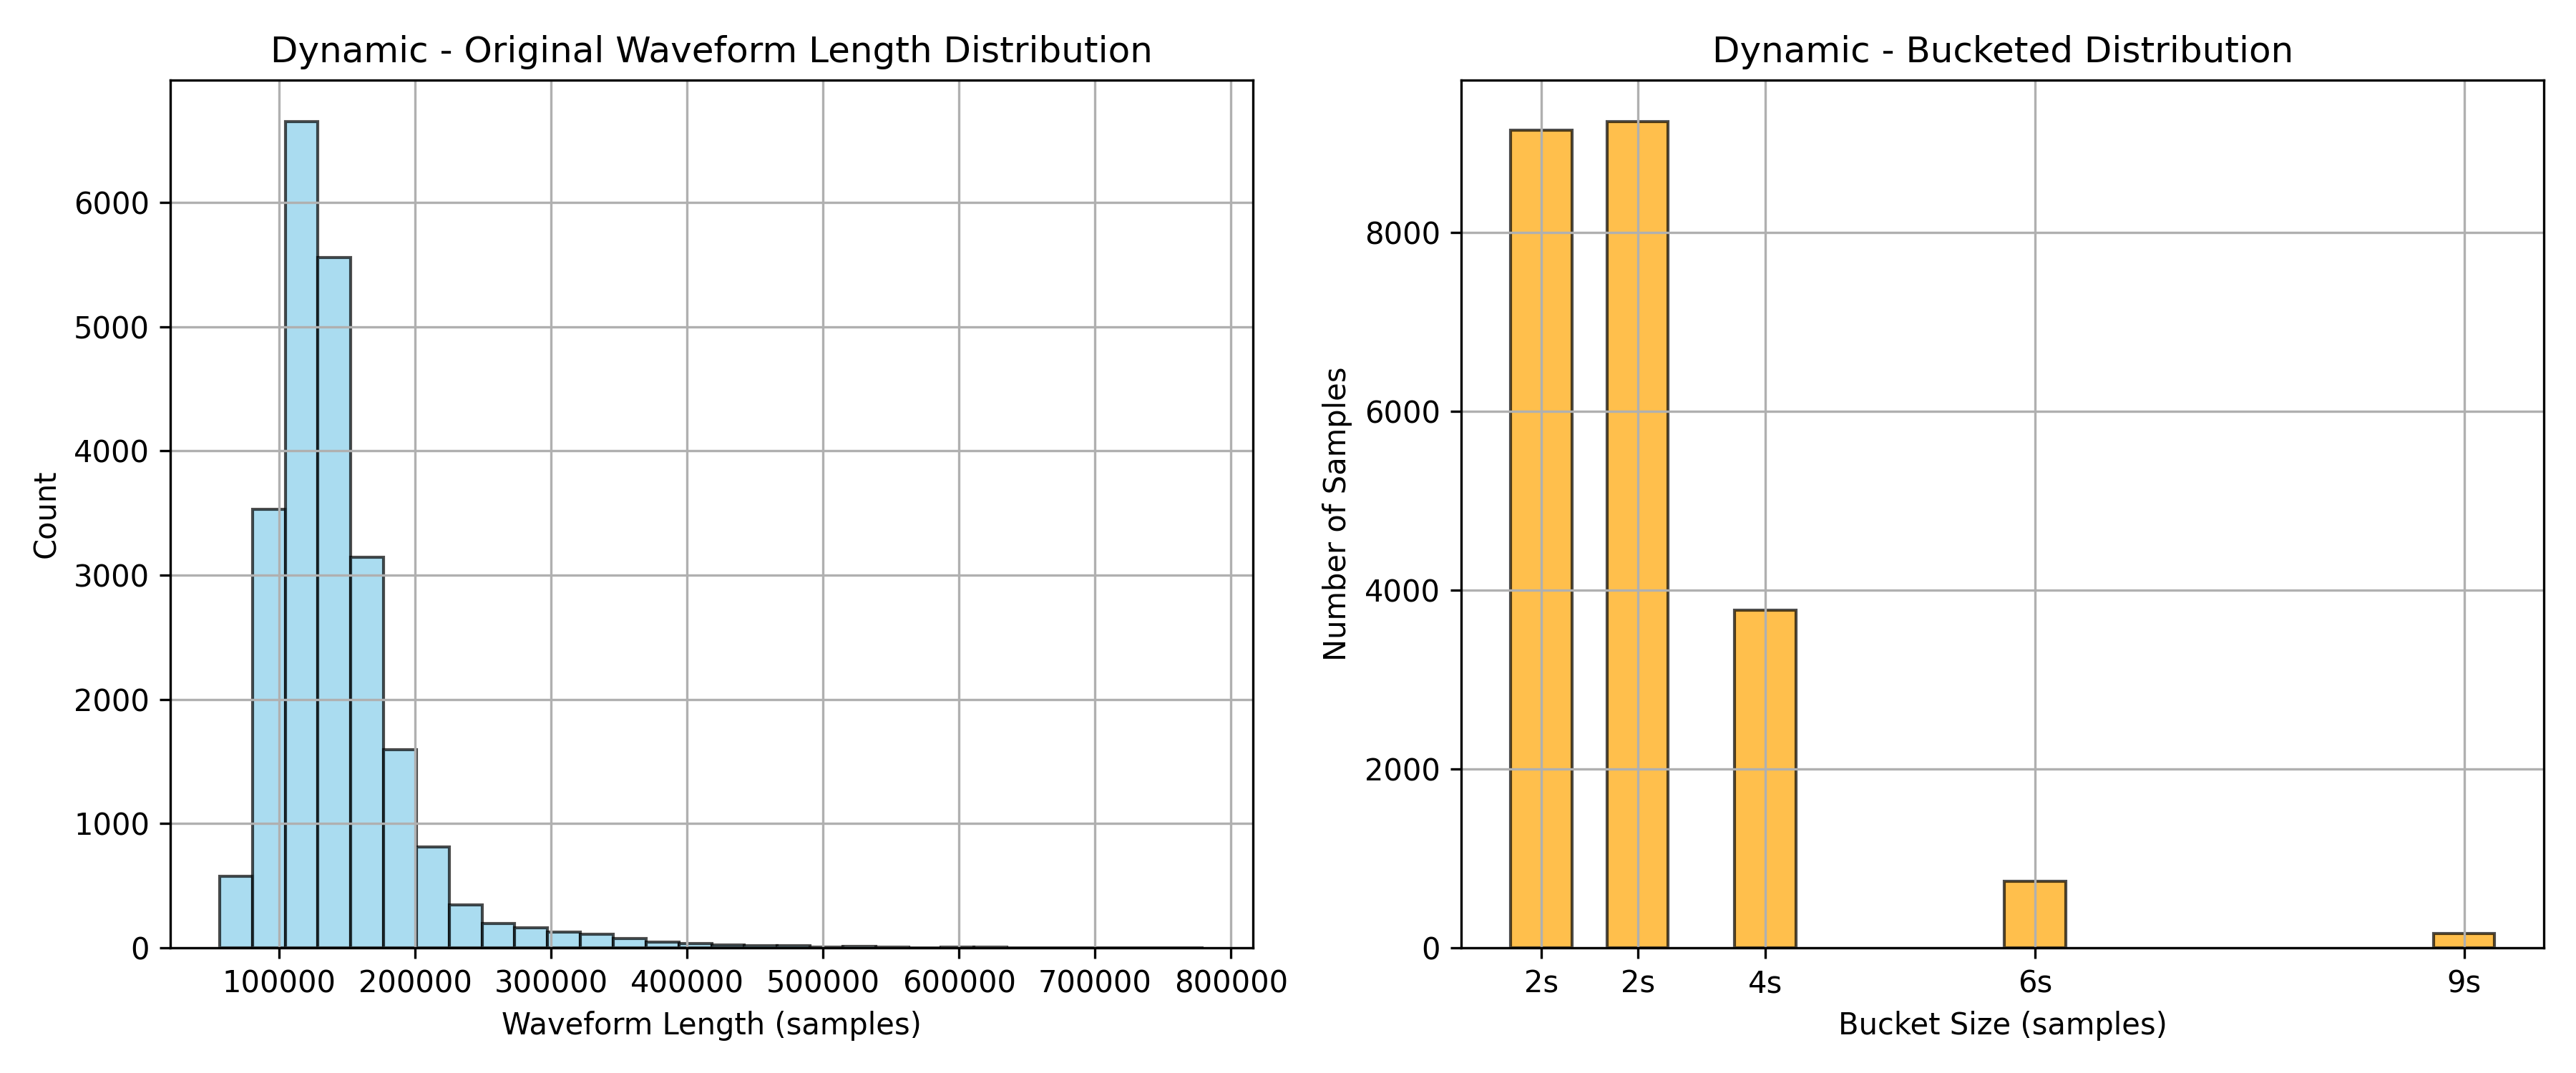
\includegraphics[width=0.9\textwidth]{dynamic_pad.png}
    \caption{Dynamic bucketing histogram and bucket allocation}
    \label{fig:dynamic_pad}
\end{figure}

The \texttt{collate} method then pads or truncates each waveform to its bucket's target size. Compared to static bucketing, dynamic bucketing leads to tighter groupings, minimizing the average amount of padding per batch. This results in better memory utilization and more efficient training.

Dynamic bucketing combines flexibility with performance, adapting to the dataset rather than imposing fixed constraints. It is particularly effective when the data contains a wide or uneven distribution of sequence lengths. When comparing dynamic to static bucketing, we observe that the dynamic method identifies two buckets around the 2-second mark that are heavily populated—clearly illustrating its ability to adapt to the underlying structure of the dataset more effectively than the fixed approach.

\subsection{Padding-Truncation Output-Truncation (PTO)}
\label{subsec:pto_dataset}

The Padding-Truncation Output-Truncation (PTO) approach avoids both fixed-length and bucketing strategies. Instead, it applies padding on a per-batch basis, using the longest sample in the batch as a reference. This ensures minimal padding while maintaining alignment within the batch.

The core idea is drawn from the work of Zhao et al.~\cite{applsci1004092}, which proposed an output-truncation mechanism for real-time audio processing. During training, each sample is padded to match the maximum length in the batch, and its original length is stored. After inference, the output is cropped back to the original length, ensuring alignment with the unpadded input.

\begin{figure}[H]
    \centering
    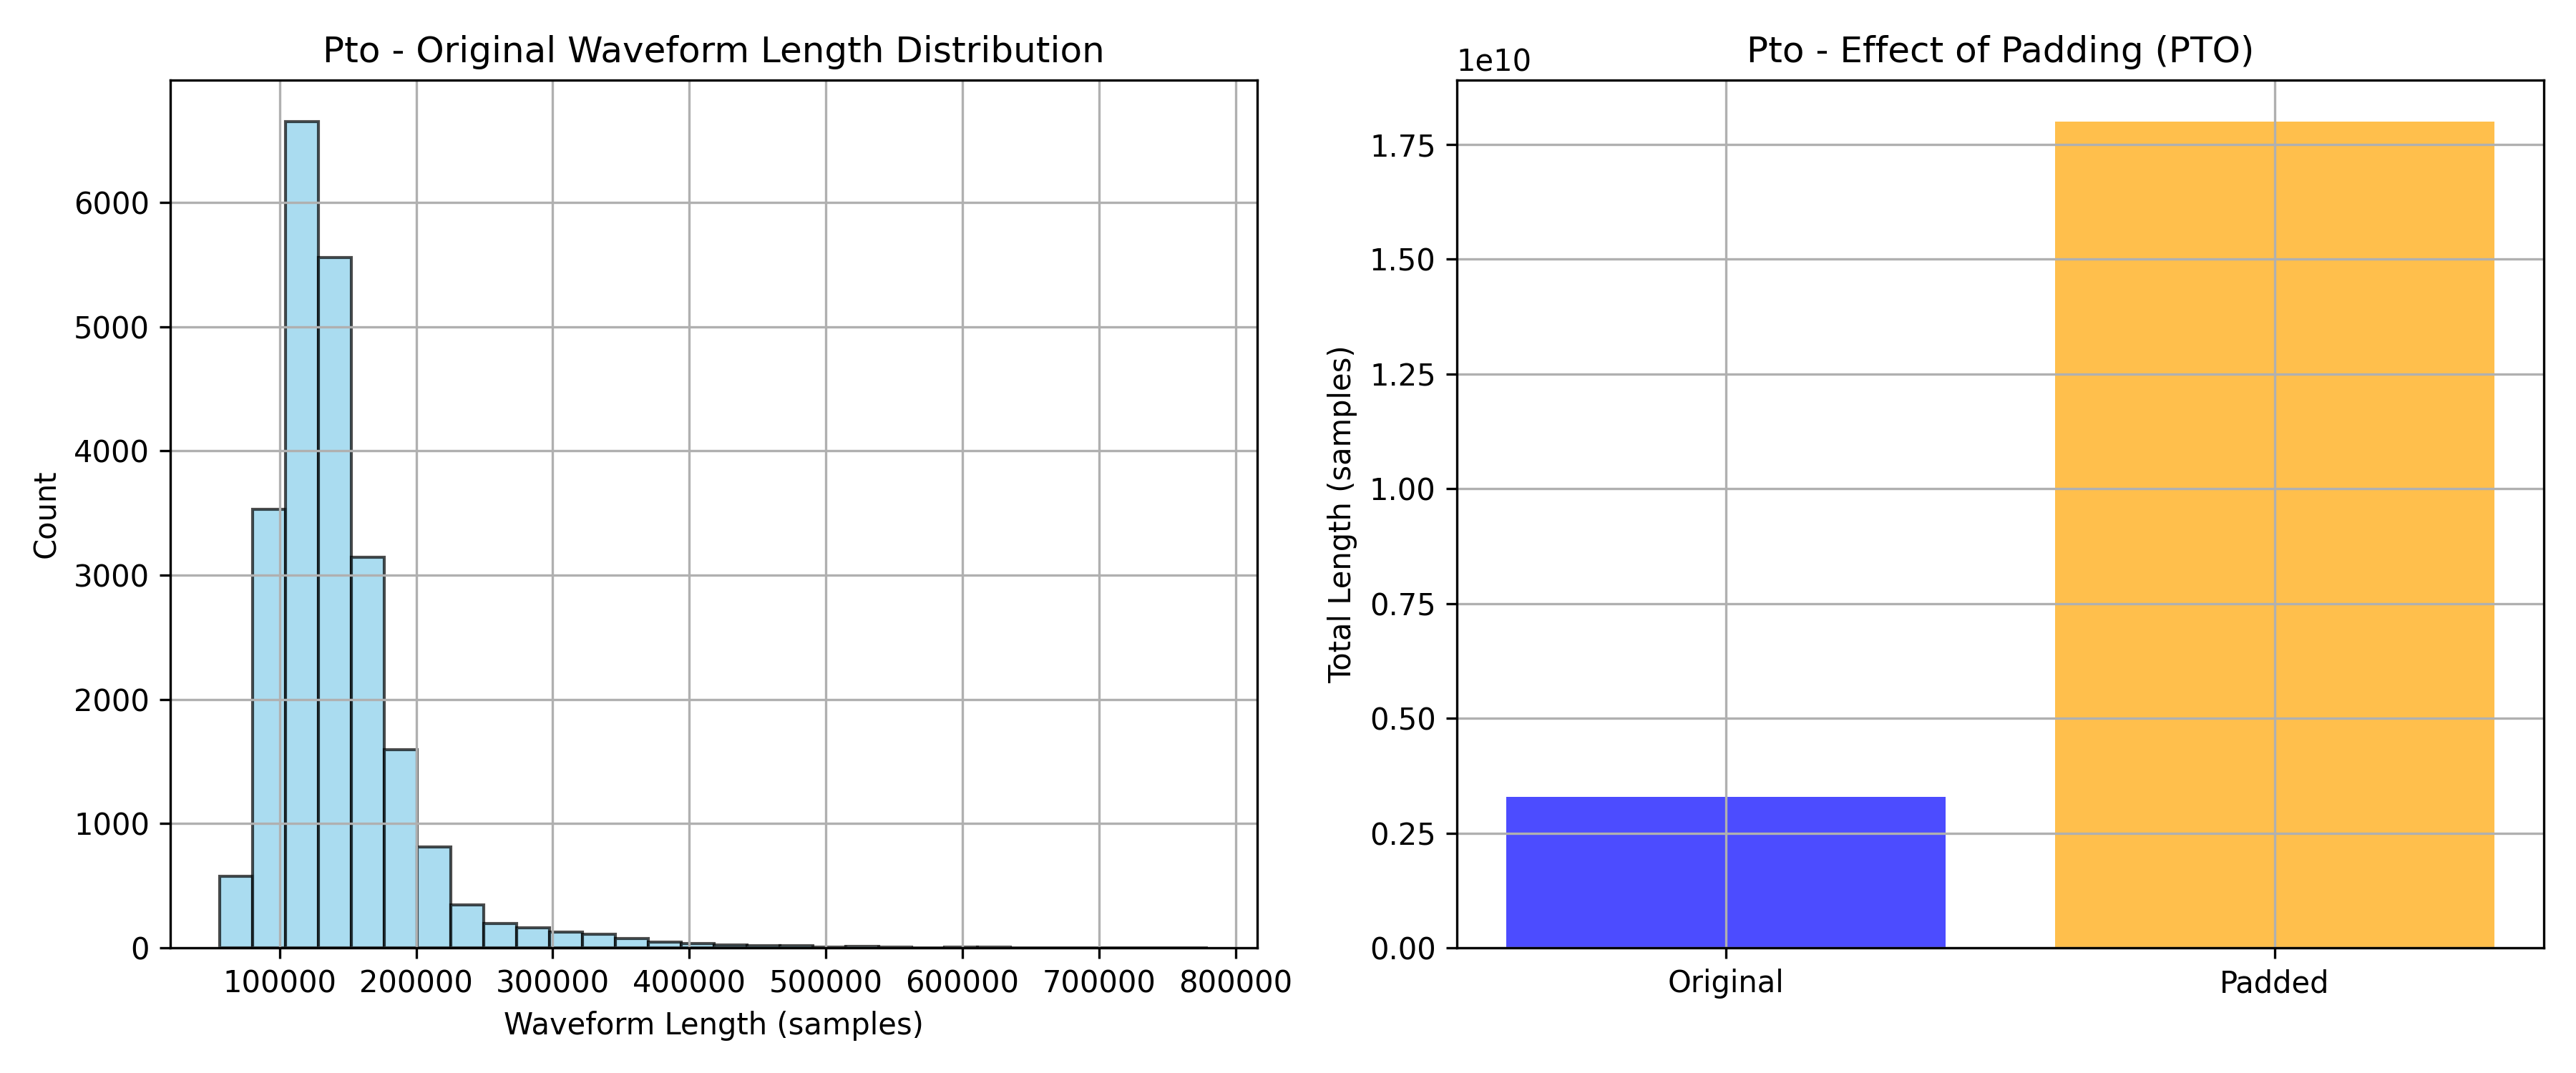
\includegraphics[width=0.9\textwidth]{pto_pad.png}
    \caption{Padding effect using the PTO method}
    \label{fig:pto_pad}
\end{figure}

In this implementation, a custom \texttt{pto\_collate} function first aligns the frequency dimension using bilinear interpolation, then pads the time axis. The model is trained on uniformly shaped tensors, but retains the ability to reconstruct clean speech at its original length, mitigating the impact of zero-padding.

The PTO method simulates real-time signal processing by training on frame-aligned STFT inputs, making it highly suitable for deployment in low-latency scenarios. Unlike bucketing methods, it does not require predefined groups or length clustering, making it the most dynamic and adaptive option in the dataset pipeline. However, it does come with its own computational overheads, as padding is still required. Furthermore, output truncation introduces an additional processing step. Although padding is mitigated at inference by truncating the output, the model is still trained on padded inputs—therefore, the cost of padding is not entirely eliminated.

\subsection{Helper Functions}
\label{subsec:helper_functions}

A few support functions are implemented to ensure that batching and visualization are handled effectively across dataset variants:

\begin{itemize}
    \item \texttt{pto\_collate}: A custom collate function used by the PTO dataset. It aligns all spectrograms along the frequency axis and pads them along the time axis, while retaining the original lengths for post-processing.
    \item \texttt{BucketSampler}: Used with static and dynamic bucketing. It ensures that batches contain only samples from the same bucket, preventing dimension mismatch during training. It randomizes batches within buckets to improve generalization.
    \item \texttt{visualize\_dataset\_padding}: A diagnostic utility that plots the distribution of original lengths and the effects of padding for each method. It provides insights into the efficiency and overhead introduced by each strategy.
\end{itemize}

\section{Out Of Memory (OOM) Handling}
\label{sec:oom_handling}

Given the depth of the model architectures and the limitations of a shared remote GPU. Out-of-Memory (OOM) errors are common when training deep learning models on constrained hardware, especially when dealing with large spectrogram tensors derived from high-resolution audio. These experienced and mitigated in implementation through several techniques employed to reduce memory footprint and ensure training stability:

\begin{itemize}
    \item \textbf{Expandable CUDA Segments:} Before initiating training, the environment variable \texttt{PYTORCH\_CUDA\_ALLOC\_CONF=expandable\_segments:True} is set. This enables PyTorch’s new memory allocator with segment expansion, which helps alleviate fragmentation issues and allows the allocator to resize memory segments dynamically. This is the first suggestion from the PyTorch documentation for OOM errors.

    \item \textbf{Mixed Precision Training:} Automatic mixed precision (AMP) was used via PyTorch’s \texttt{autocast()} and \texttt{GradScaler}. This allows intermediate tensors to be stored in 16-bit floating point (FP16) format, reducing memory usage and increasing throughput, while maintaining model weights and gradient computations in 32-bit (FP32) for stability. Figure~\ref{fig:fp16_vs_fp32} illustrates the reduced bit-width and structure of FP16 compared to FP32, highlighting the potential for nearly half the memory usage in forward and backward passes~\cite{mindspore_mixed_precision}. This approach significantly extends the trainable capacity of a model under constrained GPU environments.

    \item \textbf{Gradient Accumulation:} Since memory limitations restricted the feasible batch size, gradient accumulation was implemented to simulate larger effective batch sizes. By accumulating gradients over multiple mini-batches and only updating model weights every \texttt{accumulation\_steps} iterations, the training process maintains the same learning dynamics as a larger batch size without requiring the memory for it. This technique proved essential for deeper models like the RCED and ConvTasNet.

    \item \textbf{Manual Memory Management:} To ensure memory is cleared between epochs and reduce fragmentation, memory cleanup routines are explicitly called at the start of every epoch: \texttt{gc.collect()}, \texttt{torch.cuda.empty\_cache()}, and \texttt{torch.cuda.reset\_peak\_memory\_stats()}. This manual intervention is particularly beneficial in a shared GPU setting, where residual allocations from other users or previous epochs may linger.

    \item \textbf{Gradient Clipping:} To prevent exploding gradients, which can rapidly consume memory, gradient norms were clipped using \texttt{torch.nn.utils.clip\_grad\_norm\_()}. This maintains training stability and prevents sudden memory spikes during backpropagation, which is especially important when using high learning rates or unregularized architectures.

    \item \textbf{Learning Rate Scheduling:} An optional scheduler progressively lowers the learning rate using a step-decay approach. This helps reduce volatile updates later in training, smoothing out the optimization process and reducing the likelihood of erratic memory usage. The sheduler also saves on resources, especially in the cases when smaller models saturate at earlier epochs.

    \item \textbf{Memory Profiling:} At the end of each epoch, GPU memory statistics are logged using \texttt{torch.cuda.max\_memory\_allocated()} and \texttt{torch.cuda.max\_memory\_reserved()}. This aids in profiling memory behavior and catching potential leaks or inefficiencies across training epochs. 
\end{itemize}

\begin{figure}[H]
    \centering
    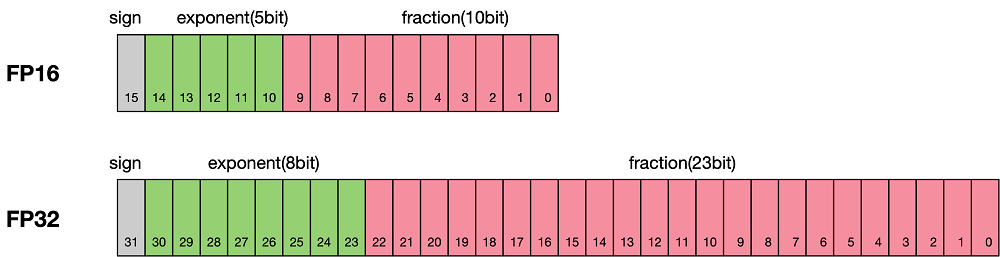
\includegraphics[width=0.9\textwidth]{fp16_vs_fp32.png}
    \caption{Comparison of memory allocation structure between FP16 and FP32 formats \cite{mindspore_mixed_precision}.}
    \label{fig:fp16_vs_fp32}
\end{figure}

These combined methods provided the foundation for training deep models across all dataset variants with minimal interruptions. Even with GPU constraints, these optimizations enabled stable, high-performance training and evaluation of multiple architectures, supporting both experimentation and reproducibility in a limited computing environment.

\section{Denoising Metrics}
\label{sec:denoising_metrics}

The denoising pipeline is just as critical as the training pipeline. Even if a model is trained effectively on high-quality data, improper evaluation or denoising procedures can lead to misleading results. This system supports both single-file inference (to output a denoised waveform) and batch processing (to compute objective evaluation metrics). Both deep learning and classical DSP approaches are supported, with behavior controlled via configuration flags and parameters.

To ensure fairness and reproducibility, all evaluations are conducted using standardized methodologies and widely adopted libraries wherever available. The following subsections outline the metrics used in the denoising pipeline to evaluate model performance.

\subsection{Signal-to-Noise Ratio (SNR)}
\label{subsec:snr}

Signal-to-Noise Ratio (SNR) measures the strength of the target signal relative to the background noise. It is defined as:

\begin{equation}
\text{SNR (dB)} = 10 \cdot \log_{10} \left( \frac{\| s \|^2}{\| s - \hat{s} \|^2} \right)
\end{equation}

where $s$ is the clean reference signal and $\hat{s}$ is the denoised signal. A higher SNR implies better denoising. In this project, SNR is computed using built-in PyTorch functions and is used as a fast, real-time-friendly performance indicator during validation and evaluation.

\subsection{Mean Squared Error (MSE)}
\label{subsec:mse}

Mean Squared Error (MSE) quantifies the average squared difference between the clean and denoised signals:

\begin{equation}
\text{MSE} = \frac{1}{N} \sum_{i=1}^{N} (s_i - \hat{s}_i)^2
\end{equation}

Although it does not correlate strongly with perceived audio quality, MSE remains a reliable signal fidelity measure and loss function. In this project, it is used to evaluate both real and imaginary components of STFT-transformed signals via \texttt{torch.nn.functional.mse\_loss}.

\subsection{Perceptual Evaluation of Speech Quality (PESQ)}
\label{subsec:pesq}

PESQ is a perceptual model developed to evaluate speech quality by simulating the human auditory system. Standardized by ITU-T in Recommendation P.862~\cite{pesq_metric}, PESQ scores range from 0 (poor) to 4.5 (excellent) and are widely used in speech enhancement and telephony.

PESQ is computed as:

\begin{equation}
\text{PESQ} = f(s, \hat{s})
\end{equation}

where $f$ is the perceptual transformation that compares the clean and denoised signals.

In this project, PESQ is computed using the \texttt{pesq} Python library in wideband mode. Since the library requires inputs to be sampled at 16 kHz, all signals are resampled from the dataset's native 48 kHz using \texttt{torchaudio.transforms.Resample} prior to evaluation.

\subsection{Short-Time Objective Intelligibility (STOI)}
\label{subsec:stoi}

STOI is designed to estimate speech intelligibility, particularly in noisy conditions. It compares time-aligned short-time spectral envelopes of clean and denoised signals and outputs a score between 0 and 1, with higher scores indicating better intelligibility.

\begin{equation}
\text{STOI} = g(s, \hat{s})
\end{equation}

The implementation used in this project is based on the open-source \texttt{pystoi} library, which adheres closely to the official MATLAB reference implementation.

\textbf{Note:} Like PESQ, STOI also requires inputs to be sampled at 16 kHz. Resampling is performed using \texttt{torchaudio.transforms.Resample} prior to computation to ensure compatibility and accurate results.

\subsection{Log Spectral Distance (LSD)}
\label{subsec:lsd}

Log Spectral Distance (LSD) measures the divergence between the log-magnitude spectra of clean and denoised signals. It captures frequency-specific distortions, making it particularly useful for evaluating audio quality in the spectral domain:

\begin{equation}
\text{LSD} = \frac{1}{F} \sum_{f=1}^{F} \sqrt{ \frac{1}{T} \sum_{t=1}^{T} \left( \log S(f, t) - \log \hat{S}(f, t) \right)^2 }
\end{equation}

where $S(f, t)$ and $\hat{S}(f, t)$ represent the magnitude spectrograms of clean and denoised signals, respectively. Since no standard library implementation exists, LSD was implemented from scratch using PyTorch tensor operations.

\vspace{1em}
In summary, these metrics collectively provide a comprehensive evaluation framework by capturing signal fidelity (SNR, MSE), perceptual quality (PESQ), intelligibility (STOI), and frequency-domain accuracy (LSD).

